\documentclass{article}
\usepackage[utf8]{inputenc}
\usepackage{graphicx}

\title{Assignment 4: CSP}
\author{Avery Frankenberg}
\date{January 28 2019}

\begin{document}

\maketitle

\section{Introduction}
For this assignment, we were tasked with creating a general constraint satisfaction problem solver (CSP). This solver has to work with multiple types of problems, both a map coloring problem and a circuit board layout problem. To implement the solver, I started by creating a CSP class and a MapColoringCSP that extends the CSP class.

\section{CSP class}
The CSP class I created has an initialization method which contains the domain values in a set, a dictionary called original assignment where every variable has all possible values associated with it, and a constraint dictionary which maps tuples of variables to legal values. These three elements are all set when the CSP is initialized by another class, for example by the MapColoringCSP class. The backtracking search method initializes the assignment dictionary and passes it to the recursive backtrack method which does the bulk of the constraint satisfaction problem solving. In the backtrack method, the assignment is returned if is complete, i.e. if all variables have one consistent, legal value. Otherwise, an unassigned variable is chosen, every value is tested and if it is consistent it the backtrack search is recursively called on this new assignment dictionary. In this way the search continues until the assignment is complete and consistent. 

Three important helper methods are the select unassigned variables method, the order values method, and the consistent method. The select unassigned variables method started out by just returning the next variable in the list that was not yet assigned (this will change later as improvements are made). The order values method also started out just returning a list of values in the order they were generated (this will also change later). Finally, the constraint method checks to make sure the new value and variable added to the assignment dictionary are consistent with the information already present. If there is nothing in the assignment dictionary yet, it returns true. If there is then it goes through every variable already in the dictionary, creates two tuples with the new variable and old variable (one with each element first) and checks that the values associated with these exist in the constraint dictionary provided to the CSP. If for any variable already in the assignment graph this is not true, the method returns False and a new value is tried. 

\section{MapColoringCSP class}
This class extends the CSP class to create the specific Map Coloring problem. It's initialization method takes three elements, a values list in words, a variables list in words and a set of tuples in words creating the constraints constraint. Then, the MapColoringCSP processes this information and turns the information it into numbers that are assigned to a values list, an original assignment dictionary, and a constraints dictionary. The convert num, convert variable, convert constraints, get not constrained, and get constrained methods all help in the conversion from the problem statement in words to numbers that can then be input into the general CSP solver. 

To run and solve the map coloring problem, the output method is run. This method calls the generateCSP method which initializes an instance of the CSP class specific to the map coloring problem. It then conducts the backtracking search and returns the final assignment. The output method takes this final assignment set and converts it back to words which it then prints to the console.

\section{CircuitBoardCSP class}
This class also extends the CSP class to create the specific Circuit Board problem. It's initialization method takes two elements, the size of the board and a dictionary that maps characters to the size of the component. The CircuitBoardCSP processes this information and turns it into numbers thus initializing values, variables, and constraints variables stored in the class. The generate num, generate values, create constraints, and get legal values methods all aid in the process of converting the problem statement into a form that can be input into the general CSP solver.

The values are generated by looping through all possible locations on the board and adding the tuples to a list. The variables are converted to numbers by simply looping through the length of the variable dictionary that is input and adding an index to a variable list for every one. This creates a variable list like the following [0, 1, 2, 3]. The constraints are generated by using both the create constraints method and the get legal values method. First, the create constraints method initializes an empty dictionary which will be subsequently filled in. By using two while loops it loops through all pairs of variables. For each pair of variables it generates the legal values. It then assigns this legal values set to be the value associated with the key, which is the tuple of two variables.  

The generate legal values method is the aspect of the constraint that ensures that two components don't overlap. This method passes two variables into a get legal values method. For every pair of locations on the board, the method gets the low and high values for both the x and y values for each of the two variables. This means it is using the location on the board as the low x and low y and then adding the width and height of piece to that location to get the high x and high y. After generating these values it starts by ensuring that neither piece goes off of the board. Then it checks to make sure that the low x value of one is greater than or equal to than the high x value of the other. It does the same for the y variable, ensuring that the low y value of one is greater than or equal to the high y value of the other. These two if statements check to make sure that the two pieces are both on the board and that they are not overlapping. 

To run and solve this problem, the output method is run. This method calls the generateCSP method in the CircuitBoardCSP class which initializes an instance of the CSP class specific to this problem. It conducts the backtracking search and returns the final assignment. This final assignment in addition to the initial problem information is passed into the final list method. The final list method converts the numbers in the final assignment into string representations of each row of the board. A list of these strings is returned to the output method and printed to the console for relatively easy viewing. In this way, this specific CSP problem extends and uses the general CSP solver just as the map coloring problem does. 

To calculate the domain of a variable with component size w x h on a board with size n x m, first we have to ensure that w is less than or equal to n and h is less than or equal to m (i.e. that the piece actually fits on the board both in the x and y directions. Then the domain of the x location of the piece is (0 : n-w) and the domain of the y location of the piece is (0 : m - h). 

\section{MAC-3 Technique}
The MAC-3 algorithm is an arc checking inference step that we can disable or enable in our algorithm by using the inf bool value. The benefits of inference is that every time a value is set in backtracking search, the possible domains are updated so that less checking has to occur in the future. It is an efficient form of forward checking. The way my algorithm works is if the inf bool value is True, indicating that we do want to use inference, the mac 3 method (maintaining arc consistency) is called on the variable, value and assignment. This method checks all of the arcs that are unassigned variables of the variable that is passed in, the one that we just assigned. The generate arc method generates the list of these neighboring arcs by retrieving the variables from the inference dictionary (a pre-processed dictionary containing the information of which variables are connected/constrained by each other) and then removing the variables that are already in the assignment. After getting this queue, the algorithm loops through every variable in the queue by popping it off, checking to see if anything needs to be revised, revising it if it does (in the revise method) and then returning. If something in this process fails, i.e. if there are no valid consistent domains remaining, then the method returns False and the backtracking algorithm knows to stop searching that path. If it returns True because the revisions are still valid then we can continue with our backtracking search.

To see the efficacy of this inference we can compare the time it took to run the CSP without the use of inference and with the use of inference. I chose to test this on the Circiut board problem because this was more complex, there were more initial values, and the help with inference is more apparent. Below are images from the two CSP solutions, the first is without inference and the second is with inference.  

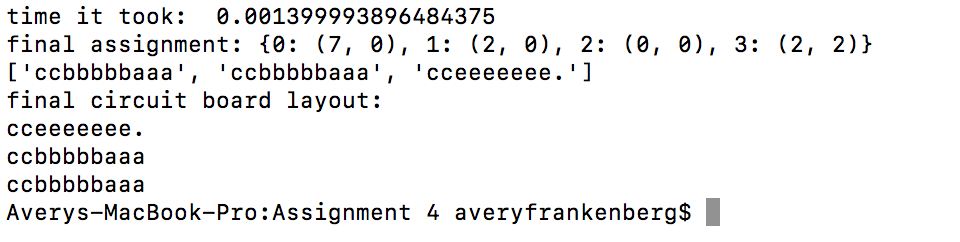
\includegraphics[width=\textwidth]{CircuitBoard_withoutInf.png}

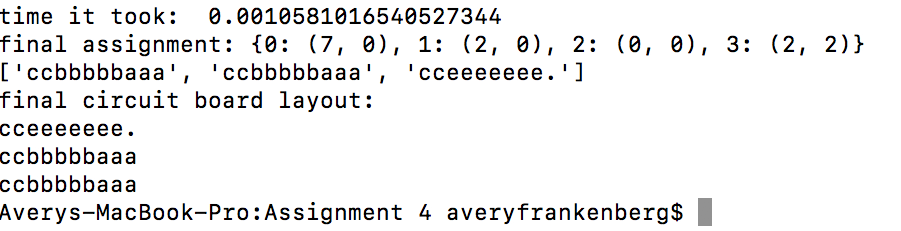
\includegraphics[width=\textwidth]{CircuitBoard_withInf.png}
We can see that the without inference it took longer to come to the solution as compared to with inference. 

\section{MRV and LCV Heuristics}
\subsection{MRV Heuristic}
The MRV (minimum remaining values) heuristic chooses to return the next variable based on how many remaining values it has in its domain. When using inference this is turned on as when inference is being done the size of the domains of each variable is changing as the algorithm progresses. When we include the MRV heuristic (by setting the naive boolean to equal False), the time spent finding a solution decrease. We can see this below, tested on the map coloring problem. The first image is without using MRV and the second is with MRV. 

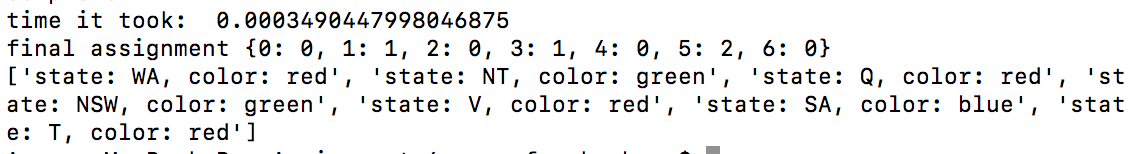
\includegraphics[width=\textwidth]{MapColor_withoutMRV.png}

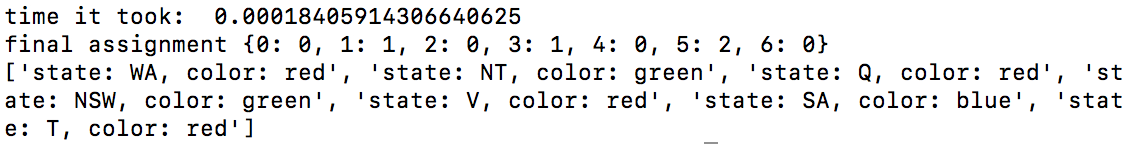
\includegraphics[width=\textwidth]{MapColor_withMRV.png}

\subsection{LCV Heuristic}
The LCV (least constraining value) heuristic helps choose which value to return first for a given variable. The idea behind it is that we want to chose the least constraining value, i.e. the value that limits the fewest domains of other variables. The way it works is if the naive boolean is False, the least constraining value method is called on the variable and assignment. For each value in the domain of that variable, it calls the forward checking method. This method counts how many subsequent domains have to change if this variable has that specific value. It then returns the count of variables changed to the least constraining value method. The lcv method takes this variables changed value and puts it into a list as a tuple (variables changed, value). After the for loop is complete, this list is sorted, putting the values that induce the fewest changes at the front, and those that induce the most at the back. Then the change values are removed and the method just returns the list of values to the backtracking method.

When we test this heuristic we can see how it decreases the amount of time the CSP solver takes. Below are two images, the first one is from running the circuit board solver normally and the second is when I run the circuit board with the LCV heuristic. 

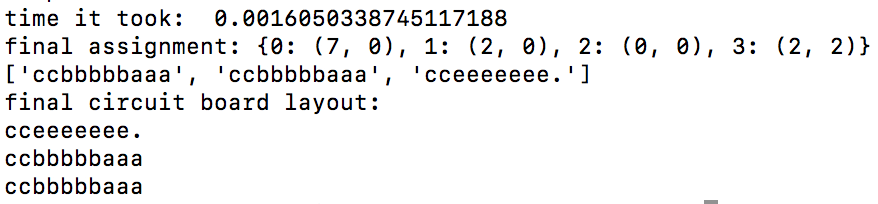
\includegraphics[width=\textwidth]{CircuitBoard_withoutLCV.png}

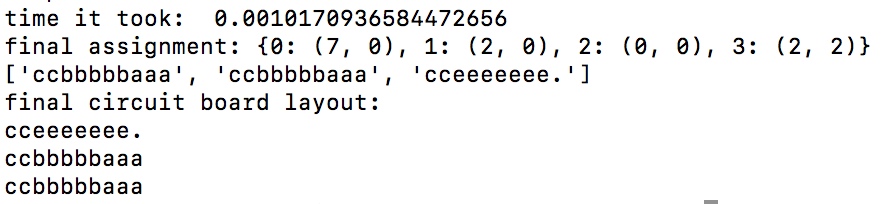
\includegraphics[width=\textwidth]{CircuitBoard_withLCV.png}

\section{Bonus}
For a bonus, I wanted to explore the current cultural and social thoughts behind constraint satisfaction problems. I want to better understand when they are used today--as map coloring problems are relatively simple--and if the way they are used changed over time. The first article that peaked my interest is from the \textit{Quanta Magazine} published in April 2018. The article is called: "First Big Steps Toward Proving the Unique Games Conjecture". This article begins by discussing the broad applicability of problems that ask some form of the question: "how do we color the nodes of a network given some rules or constraints". This question is in fact what we were working on in this project, and the article discusses how the same general thought process can be applied to the "geometry of foams and the stability of election systems". However, despite its wide applicability, the focus of this article asks about proving the conjecture that you can efficiently color networks in a specific way. The article explains how it has been established that the problem of coloring a network that requires three or more colors is NP-hard, or possibly beyond the scope of an efficient algorithm. 

The way Khot, the researcher, set out to prove the conjecture was by considering the complexity of a smaller problem--the Unique Games Problem. The goal of this problem is to color the nodes in a network based on predetermined constraints; exactly the types of problems we solved in the assignment. From this problem Khot made an additional conjecture, that "there is no efficient algorithm capable of identifying colorings, for every conceivable network, that satisfy even a tiny fraction of the number of constraints that the optimal coloring satisfies". The author describes how an interesting outcome of this conjecture is the applicability of it in different realms--for instance that semidefinite programming is the best way to solve constraint problems if the conjecture is true. 

The proof that these researchers extended is a proof of the 2-2 Games Conjecture. This 2-2 Games proof states that using broader constraints that say any node can be one of two colors, there is no efficient way to color all of the nodes in a network that satisfy even a small percentage of the constraints an optimal solution requires. The line of thinking that extends this proof is that if you can find an algorithm that satisfies almost 100 percent of the constraints in the 2-2 problem that the same algorithm could satisfy almost 50 percent in the Unique Games problem. But creating an efficient algorithm that satisfies almost 100 percent of constraints in the 2-2 game for any network is not possible. Therefore, satisfying even 50 percent of the constraints in the Unique Games problem using an efficient algorithm is also not possible.

While this proof is complicated and definitely far past the concepts we discussed in class, I find it interesting to read about and consider. It forced me to think more critically about the algorithms that I wrote. Even though MAC-3 inference, MRV, and LCV all improved the runtime--and therefore efficiency--of the search. However, after reading about these theorems and conjectures, I realized that we didn't discuss nor proving that a CSP type solution exists for all network constraint problems of this type. 

I was reading additional articles about the application of CSP problems in hospitals for patient scheduling and in these articles it talked about how there are often hard constraints and soft constraints. The hard constraints have to be satisfied but an optimal solution satisfies as many soft constraints as possible. However, as Khot's proof (could) show, and what the 2-2 Game problem proof starts to show, is that finding an efficient algorithm that satisfies all of these constriants, both hard and soft, is extremely challenging and could actually be impossible. 

Links to articles:
https://www.quantamagazine.org/computer-scientists-close-in-on-unique-games-conjecture-proof-20180424/
https://www.sciencedirect.com/science/article/pii/S095070511830025X

\end{document}
